% Options for packages loaded elsewhere
\PassOptionsToPackage{unicode}{hyperref}
\PassOptionsToPackage{hyphens}{url}
\documentclass[
  ignorenonframetext,
]{beamer}
\newif\ifbibliography
\usepackage{pgfpages}
\setbeamertemplate{caption}[numbered]
\setbeamertemplate{caption label separator}{: }
\setbeamercolor{caption name}{fg=normal text.fg}
\beamertemplatenavigationsymbolsempty
% remove section numbering
\setbeamertemplate{part page}{
  \centering
  \begin{beamercolorbox}[sep=16pt,center]{part title}
    \usebeamerfont{part title}\insertpart\par
  \end{beamercolorbox}
}
\setbeamertemplate{section page}{
  \centering
  \begin{beamercolorbox}[sep=12pt,center]{section title}
    \usebeamerfont{section title}\insertsection\par
  \end{beamercolorbox}
}
\setbeamertemplate{subsection page}{
  \centering
  \begin{beamercolorbox}[sep=8pt,center]{subsection title}
    \usebeamerfont{subsection title}\insertsubsection\par
  \end{beamercolorbox}
}
% Prevent slide breaks in the middle of a paragraph
\widowpenalties 1 10000
\raggedbottom
\AtBeginPart{
  \frame{\partpage}
}
\AtBeginSection{
  \ifbibliography
  \else
    \frame{\sectionpage}
  \fi
}
\AtBeginSubsection{
  \frame{\subsectionpage}
}
\usepackage{iftex}
\ifPDFTeX
  \usepackage[T1]{fontenc}
  \usepackage[utf8]{inputenc}
  \usepackage{textcomp} % provide euro and other symbols
\else % if luatex or xetex
  \usepackage{unicode-math} % this also loads fontspec
  \defaultfontfeatures{Scale=MatchLowercase}
  \defaultfontfeatures[\rmfamily]{Ligatures=TeX,Scale=1}
\fi
\usepackage{lmodern}
\ifPDFTeX\else
  % xetex/luatex font selection
\fi
% Use upquote if available, for straight quotes in verbatim environments
\IfFileExists{upquote.sty}{\usepackage{upquote}}{}
\IfFileExists{microtype.sty}{% use microtype if available
  \usepackage[]{microtype}
  \UseMicrotypeSet[protrusion]{basicmath} % disable protrusion for tt fonts
}{}
\makeatletter
\@ifundefined{KOMAClassName}{% if non-KOMA class
  \IfFileExists{parskip.sty}{%
    \usepackage{parskip}
  }{% else
    \setlength{\parindent}{0pt}
    \setlength{\parskip}{6pt plus 2pt minus 1pt}}
}{% if KOMA class
  \KOMAoptions{parskip=half}}
\makeatother
\usepackage{longtable,booktabs,array}
\usepackage{caption}
\captionsetup[table]{skip=6pt}
\newcounter{none} % for unnumbered tables
\usepackage{calc} % for calculating minipage widths
\usepackage{caption}
% Make caption package work with longtable
\makeatletter
\def\fnum@table{\tablename~\thetable}
\makeatother
\usepackage{graphicx}
\makeatletter
\newsavebox\pandoc@box
\newcommand*\pandocbounded[1]{% scales image to fit in text height/width
  \sbox\pandoc@box{#1}%
  \Gscale@div\@tempa{\textheight}{\dimexpr\ht\pandoc@box+\dp\pandoc@box\relax}%
  \Gscale@div\@tempb{\linewidth}{\wd\pandoc@box}%
  \ifdim\@tempb\p@<\@tempa\p@\let\@tempa\@tempb\fi% select the smaller of both
  \ifdim\@tempa\p@<\p@\scalebox{\@tempa}{\usebox\pandoc@box}%
  \else\usebox{\pandoc@box}%
  \fi%
}
% Set default figure placement to htbp
\def\fps@figure{htbp}
\makeatother
\setlength{\emergencystretch}{3em} % prevent overfull lines
\providecommand{\tightlist}{%
  \setlength{\itemsep}{0pt}\setlength{\parskip}{0pt}}
% Auto-generated by infrastructure/rendering/_pdf_latex_helpers.py::extract_math_font_preamble.
% Minimal header passed to Pandoc via -H so Beamer slides pick up the same math font
% as the combined-PDF path. Adjust the manuscript's preamble.md to change the font globally.
\usepackage{unicode-math}
\setmathfont{latinmodern-math.otf}

% Slide layout defaults for warning-clean scientific decks.
\usepackage{etoolbox}
\IfFileExists{xurl.sty}{\usepackage{xurl}}{}
\IfFileExists{seqsplit.sty}{\usepackage{seqsplit}}{\newcommand{\seqsplit}[1]{#1}}
\protected\def\breakseq#1{\seqsplit{#1}}
\protected\def\breaktt#1{\begingroup\ttfamily\seqsplit{#1}\endgroup}
\setlength{\emergencystretch}{6em}
\tolerance=5000
\hbadness=10000
\hfuzz=1pt
\setlength{\tabcolsep}{2pt}
\AtBeginEnvironment{longtable}{\tiny\renewcommand{\arraystretch}{0.86}\setlength{\tabcolsep}{1pt}}
\AtBeginEnvironment{tabular}{\tiny\renewcommand{\arraystretch}{0.86}\setlength{\tabcolsep}{1pt}}
\AtBeginEnvironment{equation}{\tiny}
\AtBeginEnvironment{equation*}{\tiny}
\AtBeginEnvironment{align}{\tiny}
\AtBeginEnvironment{align*}{\tiny}
\AtBeginEnvironment{itemize}{\footnotesize}
\AtBeginEnvironment{enumerate}{\footnotesize}
\AtBeginEnvironment{description}{\footnotesize}
\setbeamerfont{caption}{size=\tiny}
\setbeamerfont{caption name}{size=\tiny}
\setbeamerfont{normal text}{size=\small}
\setbeamerfont{frametitle}{size=\small}
\setbeamerfont{section title}{size=\footnotesize}
\setbeamerfont{subsection title}{size=\footnotesize}
\setbeamertemplate{section page}{%
  \centering
  \begin{beamercolorbox}[sep=12pt,center,wd=\paperwidth]{section title}
    \parbox{0.86\paperwidth}{\centering\usebeamerfont{section title}\insertsection\par}
  \end{beamercolorbox}
}
\setbeamertemplate{subsection page}{%
  \centering
  \begin{beamercolorbox}[sep=8pt,center,wd=\paperwidth]{subsection title}
    \parbox{0.86\paperwidth}{\centering\usebeamerfont{subsection title}\insertsubsection\par}
  \end{beamercolorbox}
}
\setlength{\abovecaptionskip}{2pt}
\setlength{\belowcaptionskip}{0pt}

% Natbib and cross-reference fallbacks — slides don't load natbib
% or cleveref, but combined-PDF manuscript prose may emit these
% commands. The fallback renders citations as a bracketed key list
% and cross-references as detokenized labels so slides don't fail on
% undefined control sequences or raw underscores. \providecommand is
% a no-op if packages load later.
\providecommand{\citep}[1]{[#1]}
\providecommand{\citet}[1]{#1}
\providecommand{\citealp}[1]{#1}
\providecommand{\citeauthor}[1]{#1}
\providecommand{\citeyear}[1]{#1}
\providecommand{\cref}[1]{\texttt{\detokenize{#1}}}
\providecommand{\Cref}[1]{\texttt{\detokenize{#1}}}

\newtheorem{proposition}{Proposition}
\newtheorem{hypothesis}{Hypothesis}
\usepackage{bookmark}
\IfFileExists{xurl.sty}{\usepackage{xurl}}{} % add URL line breaks if available
\urlstyle{same}
% fallback for those not using the hyperref driver hyperxmp:
\makeatletter
\@ifundefined{xmpquote}{\newcommand{\xmpquote}[1]{#1}}{}
\makeatother
\hypersetup{
  hidelinks,
  pdfcreator={LaTeX via pandoc}}

\author{\texorpdfstring{}{}}
\date{}

\begin{document}

\section{Results: Scholarship Coverage and Evidence-Status
Audits}\label{sec:results-scholarship-source-health-evidence}

\begin{frame}[fragile,allowframebreaks]{Citation coverage, locator
health, and evidence-class auditing}
\protect\phantomsection\label{citation-coverage-locator-health-and-evidence-class-auditing}
The manuscript's source coverage is also treated as a generated result.
Every authored citation is parsed from the section files, matched
against \texttt{references.bib}, and mapped through
\breaktt{data/scholarship\_sources.yaml} into a source lane and support
role before the build writes figures. The current audit covers 188 cited
sources; that number is generated from the manuscript and source matrix,
not maintained as a prose claim. fig.~\ref{fig:scholarship_coverage}
shows both sides of the contract: the left panel compares cited sources
with the matrixed source pool for each lane, while the right panel shows
which manuscript sections carry each lane. The audit is deliberately
orthogonal to the numeric claim registry: one gate protects computed
quantities; the other protects the scholarly support surface.
\end{frame}

\begin{frame}[fragile,allowframebreaks]{Citation coverage, locator
health, and evidence-class auditing}

\begin{figure}
\centering
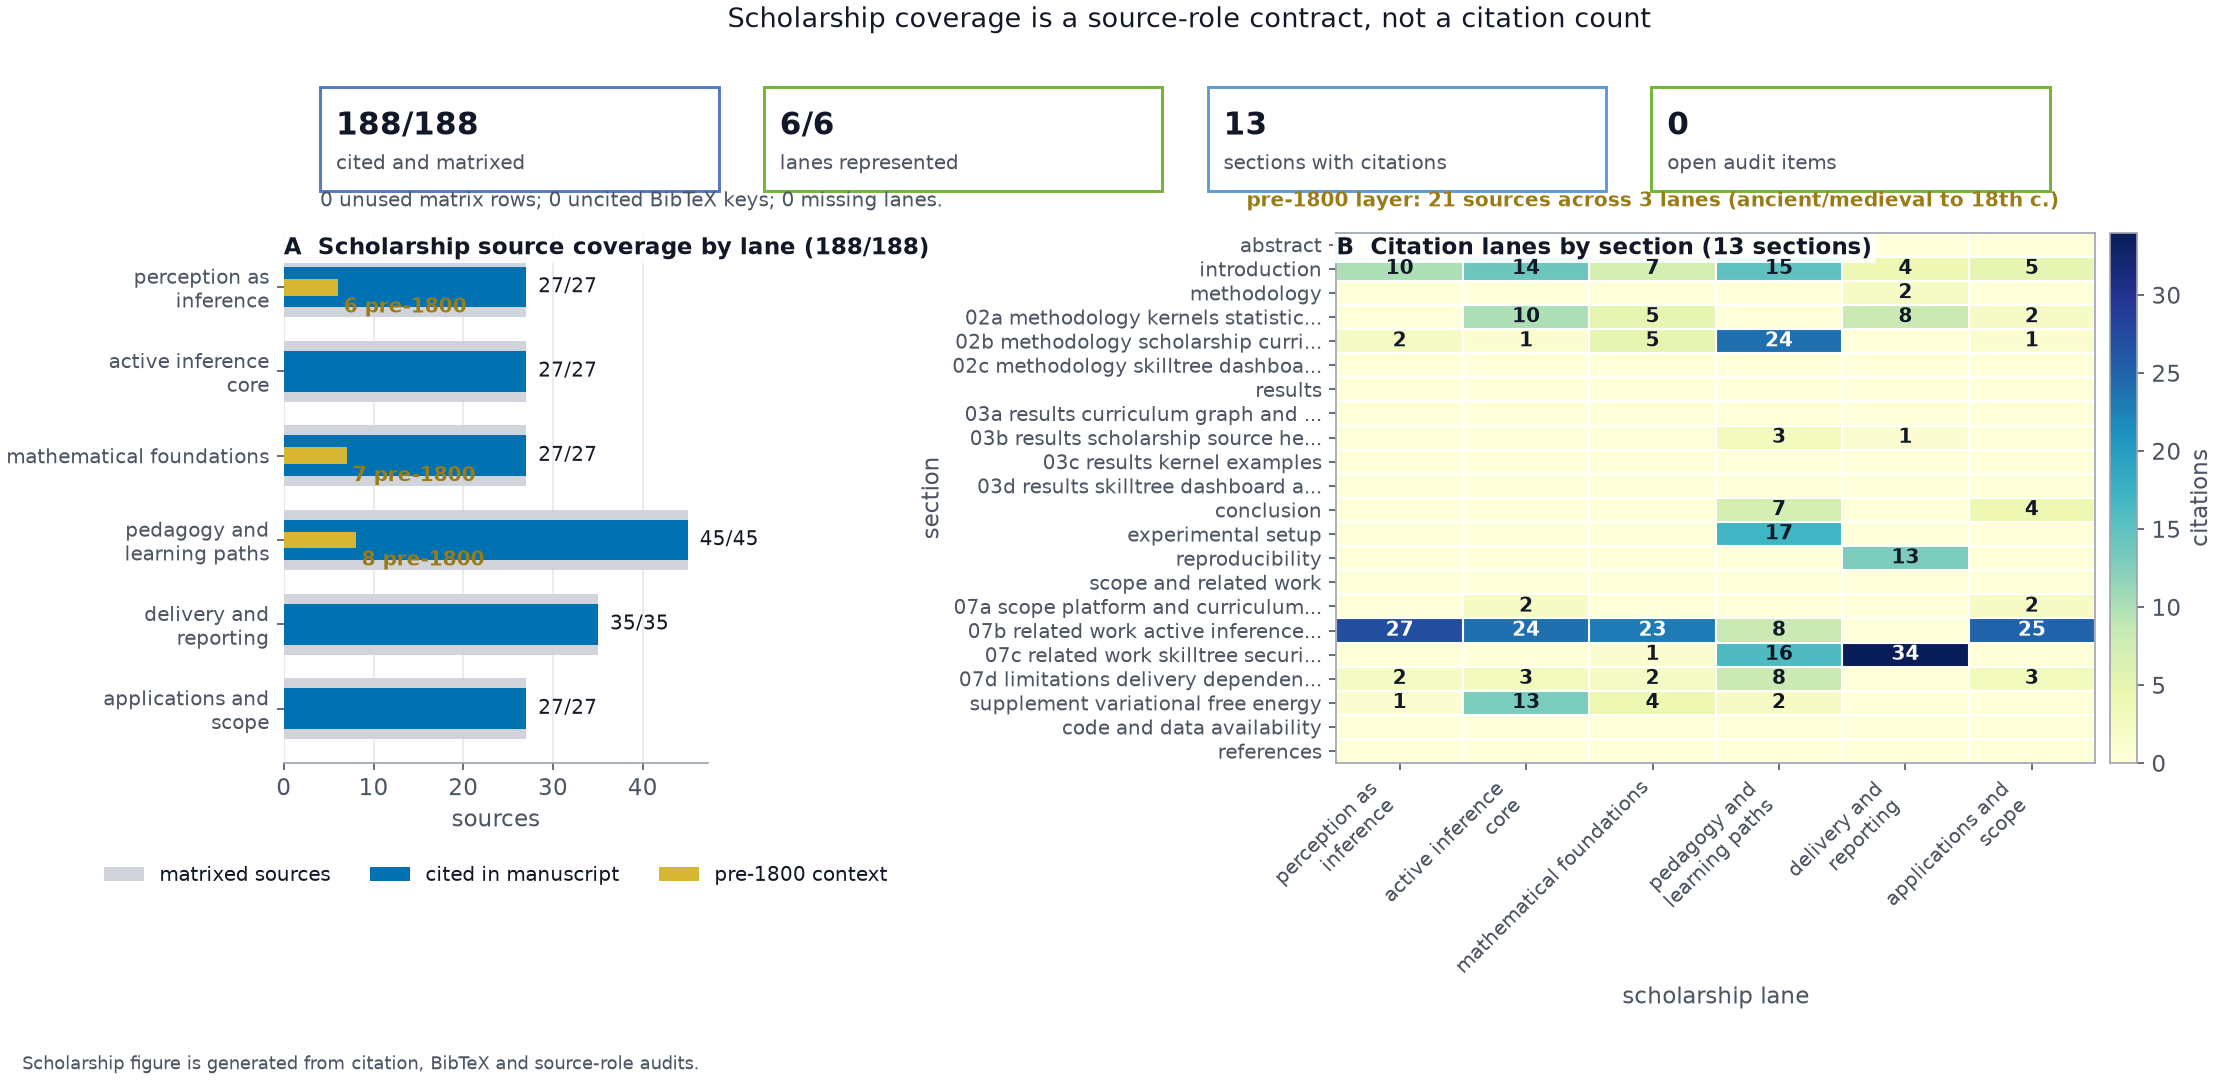
\includegraphics[width=1\linewidth,height=0.40\textheight,keepaspectratio,alt={Scholarship coverage audit generated from manuscript citations, BibTeX keys, and the source-role matrix. The left panel compares cited versus matrixed sources by scholarship lane; the right panel maps manuscript sections to citation lanes. This figure makes support distribution inspectable: a large bibliography is not treated as sufficient unless sources are cited in the sections and roles where they support specific claims.}]{../figures/scholarship_coverage.png}
\caption{Scholarship coverage audit generated from manuscript citations,
BibTeX keys, and the source-role matrix. The left panel compares cited
versus matrixed sources by scholarship lane; the right panel maps
manuscript sections to citation lanes. This figure makes support
distribution inspectable: a large bibliography is not treated as
sufficient unless sources are cited in the sections and roles where they
support specific claims.}\label{fig:scholarship_coverage}
\end{figure}

\end{frame}

\begin{frame}[fragile,allowframebreaks]{Citation coverage, locator
health, and evidence-class auditing}
The open-science education layer is also explicit. Active Skillference
cites the Active Inference Institute's public education ecosystem,
including the open-source course infrastructure, the START
curriculum-generation project, and the Institute website's open-science
educational mission (Active Inference Institute 2026b, 2026d, 2026a).
The generated local Learn material also links every exported skill to
commit-pinned external material pointers, including the Active Inference
Institute cognitive knowledge base (Active Inference Institute 2026c).
fig.~\ref{fig:open_science_sources} shows both surfaces together: cited
public sources remain visible, and the course-material source rows
expose how the cognitive knowledge base enters the generated skill
records.

\end{frame}

\begin{frame}[fragile,allowframebreaks]{Citation coverage, locator
health, and evidence-class auditing}
\begin{figure}
\centering
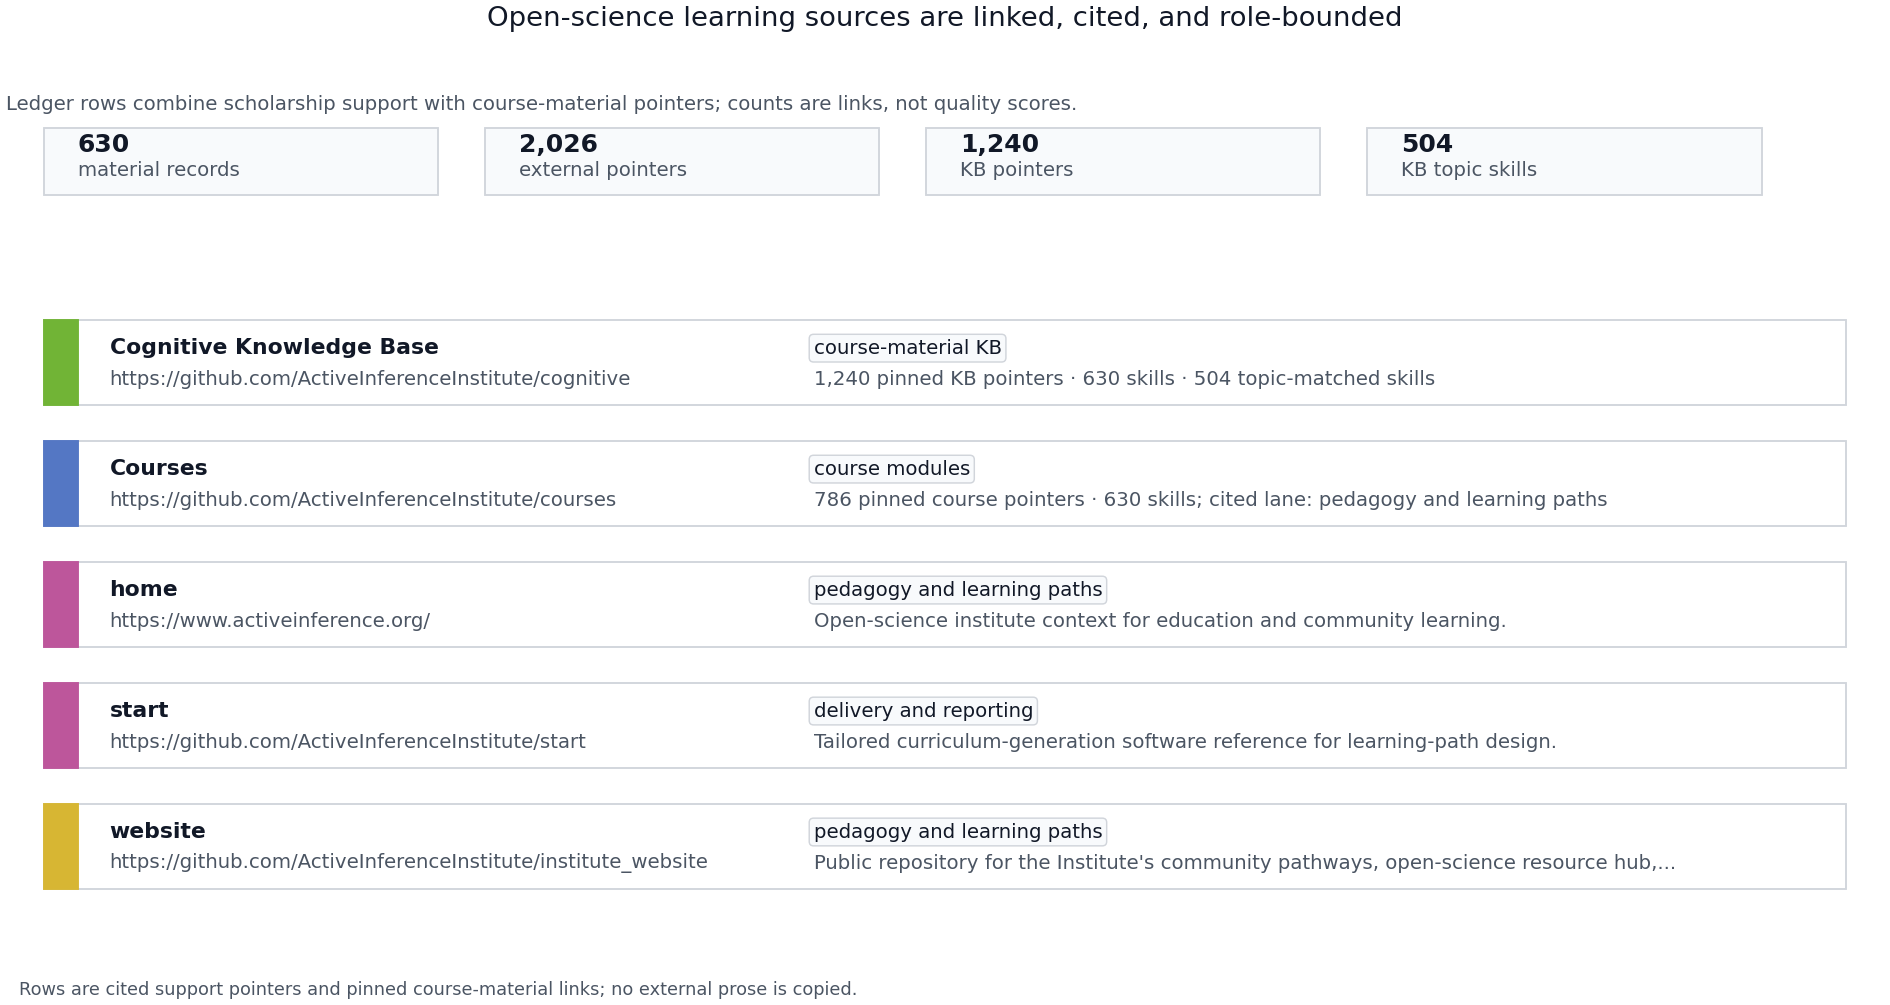
\includegraphics[width=0.88\linewidth,height=0.40\textheight,keepaspectratio,alt={Active Inference Institute open-science learning sources across scholarship support and generated course-material pointers. Summary cards report local material records, external pointers, cognitive knowledge-base pointers, and topic-matched KB skills; ledger rows distinguish the course repository, cognitive knowledge-base source, Institute homepage, website repository, and START source with locator and role text. The website repository is a community/resource-hub pointer rather than a course or knowledge-base record. The figure records pinned links and cited support surfaces; it does not claim endorsement, completeness, or copied ownership of the public education ecosystem.}]{../figures/open_science_source_map.png}
\caption{Active Inference Institute open-science learning sources across
scholarship support and generated course-material pointers. Summary
cards report local material records, external pointers, cognitive
knowledge-base pointers, and topic-matched KB skills; ledger rows
distinguish the course repository, cognitive knowledge-base source,
Institute homepage, website repository, and START source with locator
and role text. The website repository is a community/resource-hub
pointer rather than a course or knowledge-base record. The figure
records pinned links and cited support surfaces; it does not claim
endorsement, completeness, or copied ownership of the public education
ecosystem.}\label{fig:open_science_sources}
\end{figure}

\end{frame}

\begin{frame}[fragile,allowframebreaks]{Citation coverage, locator
health, and evidence-class auditing}
The source matrix is then checked a second way: source locators must be
syntactically specific, documentation entries must use URL locators, and
each support role must be substantive enough to explain why the source
is present. fig.~\ref{fig:scholarship_source_health} reports the
resulting offline source-health audit and provides a place for optional
online DOI/URL reachability checks to surface when release review
requires currentness evidence.

\end{frame}

\begin{frame}[fragile,allowframebreaks]{Citation coverage, locator
health, and evidence-class auditing}
\begin{figure}
\centering
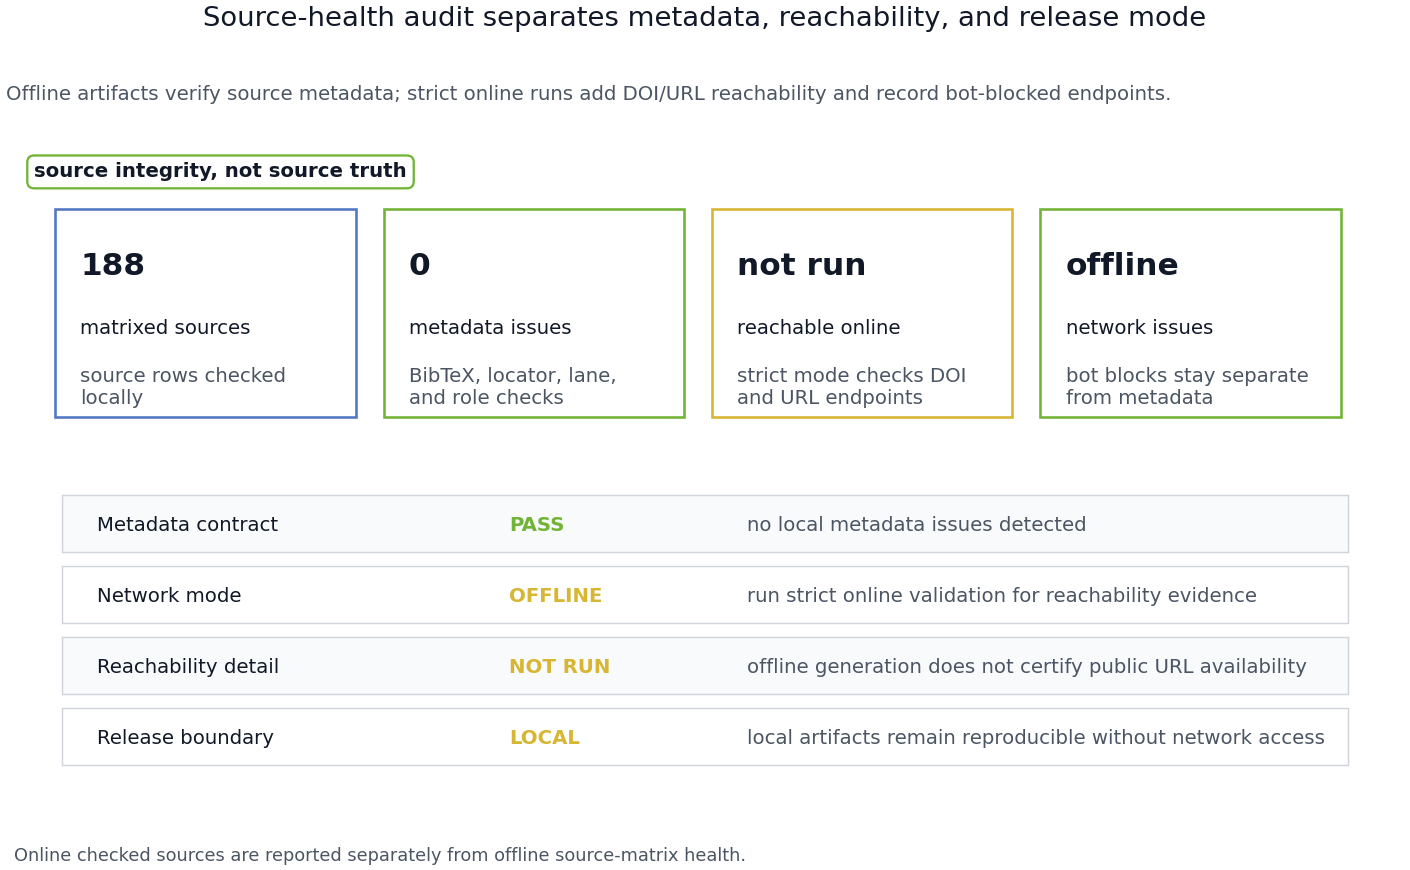
\includegraphics[width=0.88\linewidth,height=0.40\textheight,keepaspectratio,alt={Scholarship source-health audit generated from locator syntax, lane assignment, and support-role checks. Status cards separate matrixed source count, offline validation issues, and online-check mode, while the ledger rows distinguish local metadata health from optional network reachability. The figure separates two different claims: a source can be present in the matrix and still require locator, role, or currentness repair before release.}]{../figures/scholarship_source_health.png}
\caption{Scholarship source-health audit generated from locator syntax,
lane assignment, and support-role checks. Status cards separate matrixed
source count, offline validation issues, and online-check mode, while
the ledger rows distinguish local metadata health from optional network
reachability. The figure separates two different claims: a source can be
present in the matrix and still require locator, role, or currentness
repair before release.}\label{fig:scholarship_source_health}
\end{figure}

\end{frame}

\begin{frame}[fragile,allowframebreaks]{Citation coverage, locator
health, and evidence-class auditing}
The validation surface is intentionally visible rather than left as a
hidden CI detail. fig.~\ref{fig:validation_surface_matrix} summarizes
which gates bind generated JSON, negative controls, manuscript text,
dashboard artifacts, release documentation, and SkillTree handoffs. Its
count panel is rebuilt from the same graph, claim registry, scholarship
audit and roadmap state that produce the curriculum and manuscript
variables. The result is a falsifiable release claim: if a count,
citation, figure, dashboard artifact, release inventory row, or roadmap
item drifts away from its generator, the validator fails before the
manuscript or SkillTree export can be presented as current.

\end{frame}

\begin{frame}[fragile,allowframebreaks]{Citation coverage, locator
health, and evidence-class auditing}
\begin{figure}
\centering
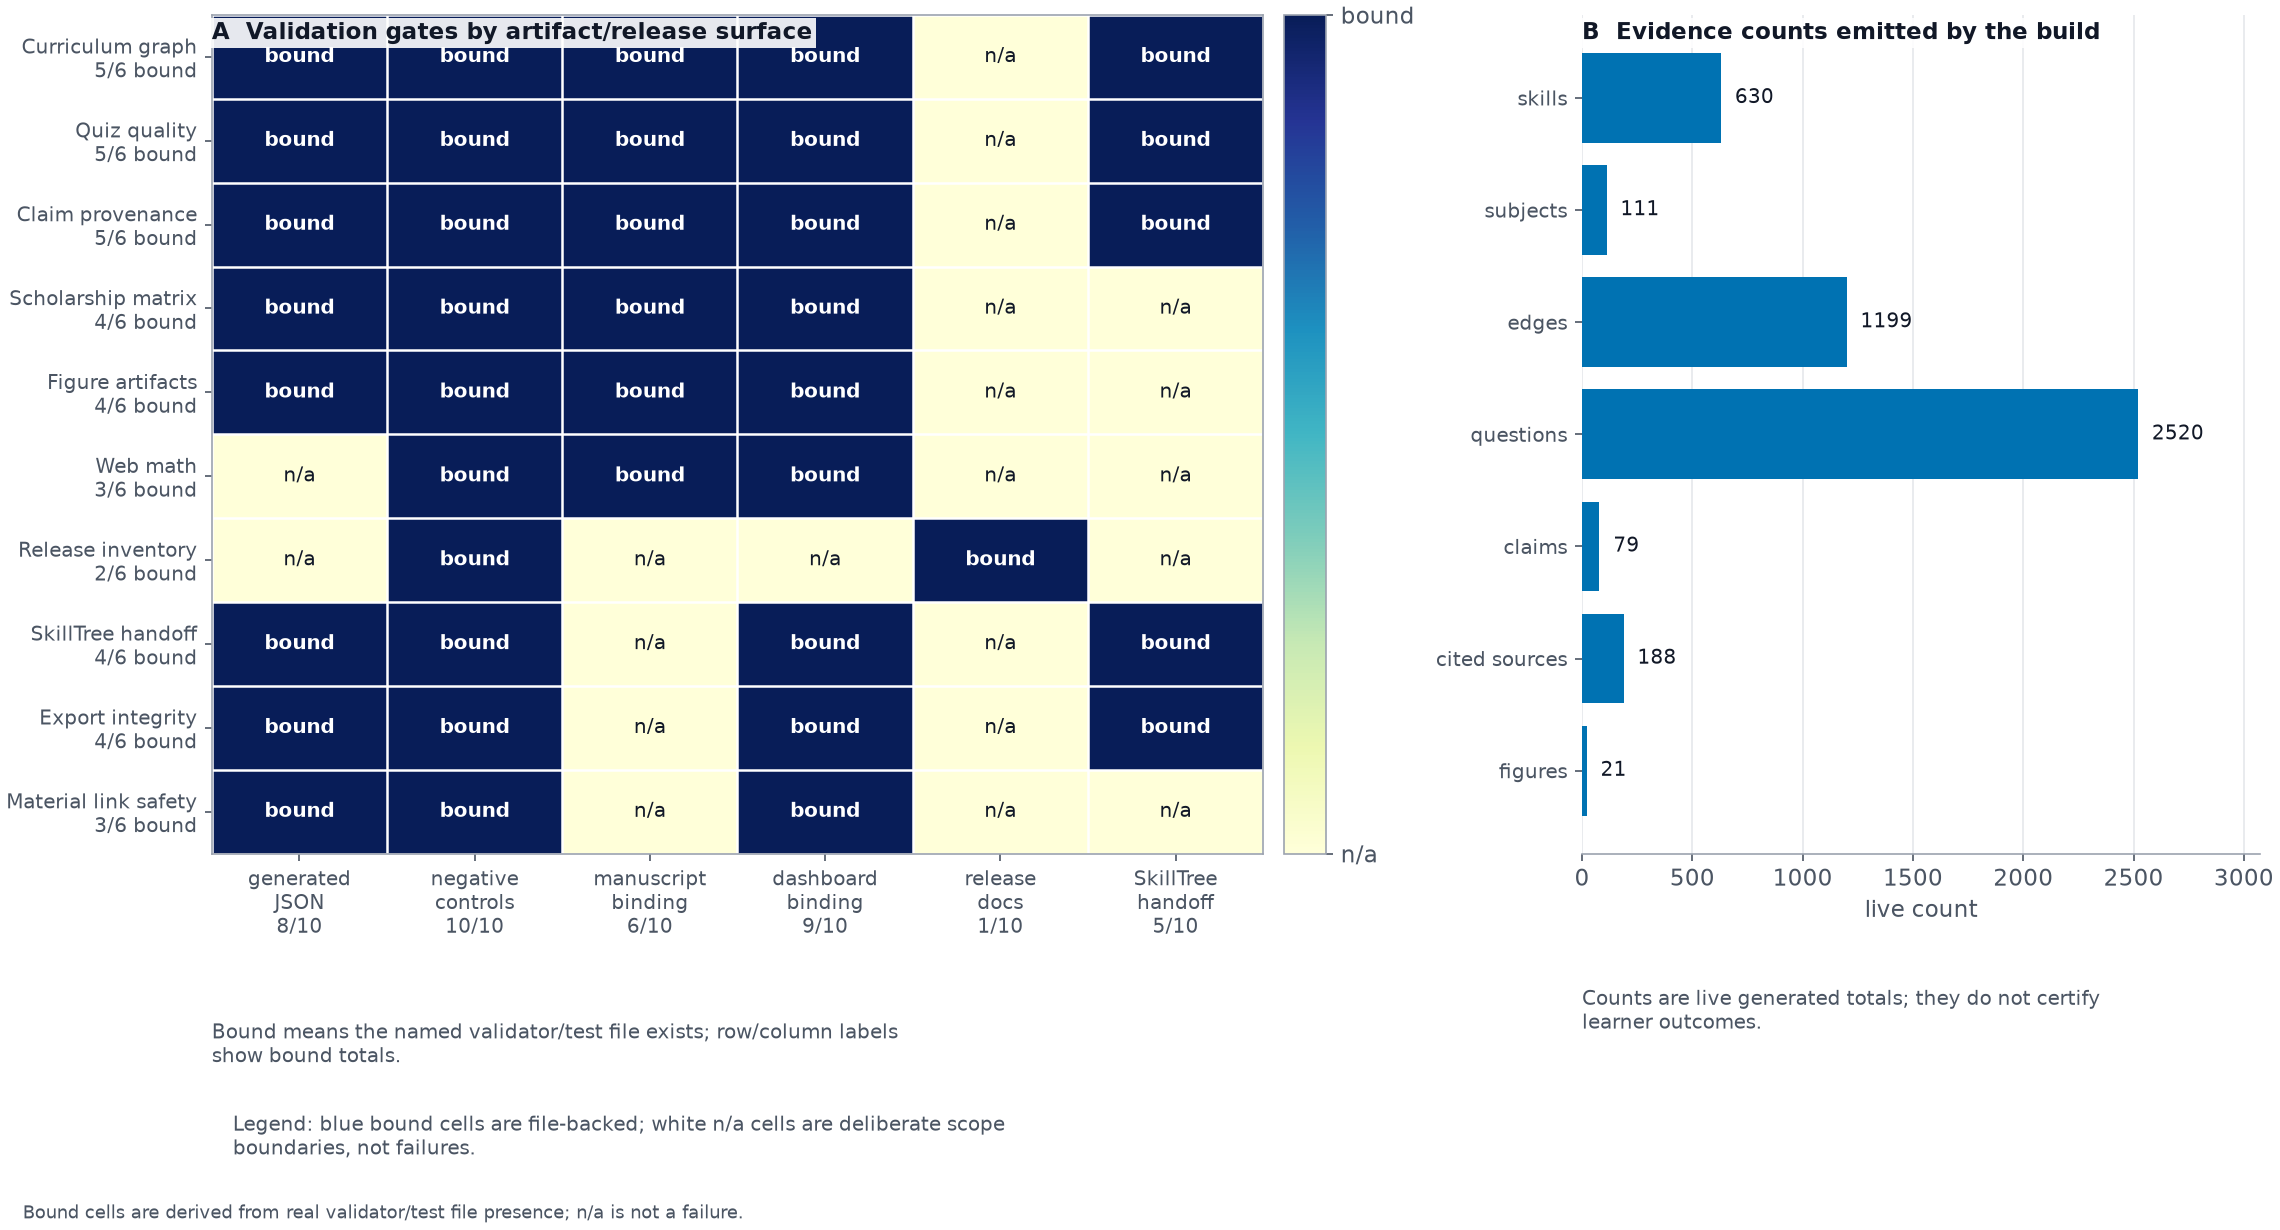
\includegraphics[width=1\linewidth,height=0.40\textheight,keepaspectratio,alt={Validation-surface matrix for Active Skillference. Each cell is derived from the on-disk presence of the validator or test file that binds that artifact surface: a cell reads ``bound'' only when every file named in its binding exists, so deleting a gate flips its cell to ``n/a'' rather than leaving a stale ``bound'' claim. Row and column labels state bound-cell totals, and each cell carries text, so the figure remains readable without heatmap color. The side panel reports live evidence counts for skills, subjects, dependencies, assessment questions, claims, cited sources, and registered figures, read directly from the graph, claim registry, scholarship audit, and figure inventory. The interpretation boundary is important: a bound cell means a named validator file exists for that artifact surface (not that the gate is guaranteed sound), while an unbound cell marks a surface that is out of scope for that gate.}]{../figures/validation_surface_matrix.png}
\caption{Validation-surface matrix for Active Skillference. Each cell is
derived from the on-disk presence of the validator or test file that
binds that artifact surface: a cell reads ``bound'' only when every file
named in its binding exists, so deleting a gate flips its cell to
``n/a'' rather than leaving a stale ``bound'' claim. Row and column
labels state bound-cell totals, and each cell carries text, so the
figure remains readable without heatmap color. The side panel reports
live evidence counts for skills, subjects, dependencies, assessment
questions, claims, cited sources, and registered figures, read directly
from the graph, claim registry, scholarship audit, and figure inventory.
The interpretation boundary is important: a bound cell means a named
validator file exists for that artifact surface (not that the gate is
guaranteed sound), while an unbound cell marks a surface that is out of
scope for that gate.}\label{fig:validation_surface_matrix}
\end{figure}

\end{frame}

\begin{frame}[fragile,allowframebreaks]{Citation coverage, locator
health, and evidence-class auditing}
fig.~\ref{fig:validation_intent_mismatch_matrix} makes the negative
controls behind that release view explicit. It separates missing
registry rows, missing files, missing manuscript labels, missing
dashboard artifacts, missing roadmap metrics, and stale manifests so the
validation layer is judged by concrete false-certification classes
rather than by the presence of a polished figure alone.

\end{frame}

\begin{frame}[fragile,allowframebreaks]{Citation coverage, locator
health, and evidence-class auditing}
\begin{figure}
\centering
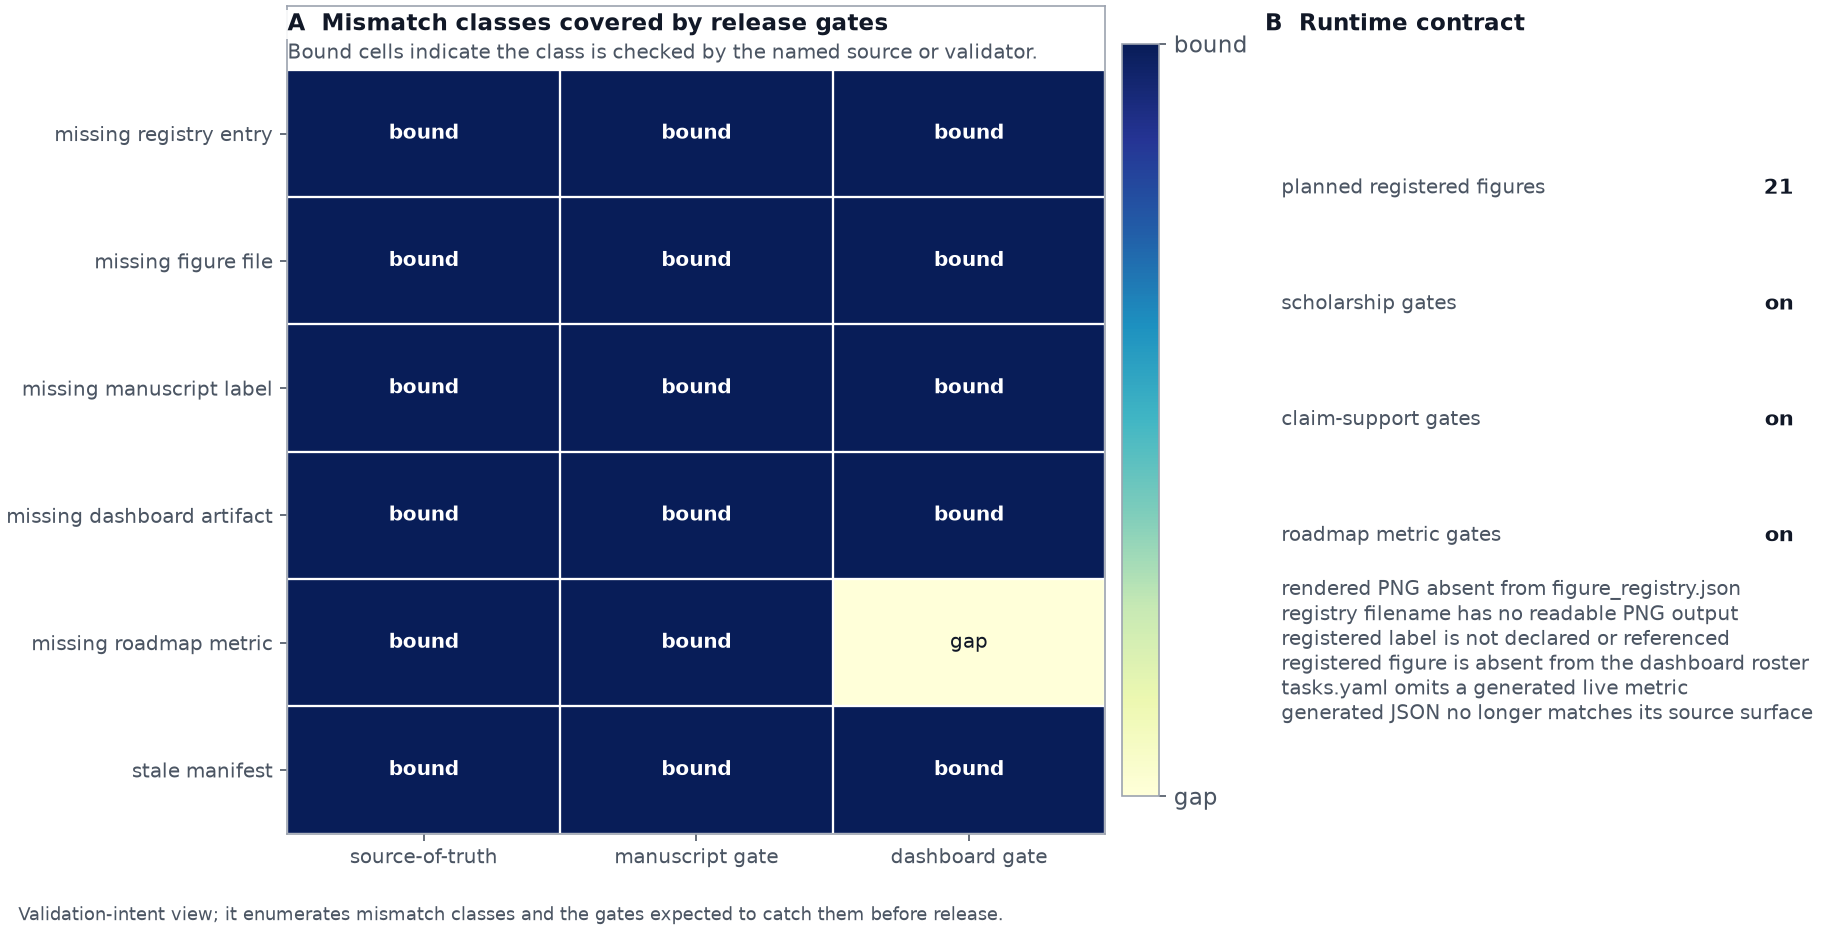
\includegraphics[width=0.98\linewidth,height=0.40\textheight,keepaspectratio,alt={Validation-intent mismatch matrix for Active Skillference. Rows enumerate concrete false-certification classes: a rendered PNG omitted from the registry, a registered figure without a readable file, a registered label omitted from the manuscript, a registered figure omitted from the dashboard artifact roster, a missing roadmap live metric, and a stale generated manifest. Columns show whether the source-of-truth, manuscript gate, or dashboard gate is expected to reject each mismatch before release. The right panel records the planned registered-figure count and which optional audit surfaces were enabled for the render.}]{../figures/validation_intent_mismatch_matrix.png}
\caption{Validation-intent mismatch matrix for Active Skillference. Rows
enumerate concrete false-certification classes: a rendered PNG omitted
from the registry, a registered figure without a readable file, a
registered label omitted from the manuscript, a registered figure
omitted from the dashboard artifact roster, a missing roadmap live
metric, and a stale generated manifest. Columns show whether the
source-of-truth, manuscript gate, or dashboard gate is expected to
reject each mismatch before release. The right panel records the planned
registered-figure count and which optional audit surfaces were enabled
for the render.}\label{fig:validation_intent_mismatch_matrix}
\end{figure}

\end{frame}

\begin{frame}[fragile,allowframebreaks]{Citation coverage, locator
health, and evidence-class auditing}
The same contract is now represented inside the curriculum rather than
only enforced at release time. The visual-evidence slice adds a
prerequisite-gated authoring path for question contracts, data grain,
encoding strength, annotation boundaries, static/mobile readability, and
negative-control validation.
fig.~\ref{fig:visual_evidence_contract_ladder} shows that path as
generated curriculum evidence: each rung names the live skill that
carries the review step, while the registry and dashboard expose the
same structured chart-contract fields. This is a deterministic
artifact-integrity claim, not a claim that the visual curriculum has
been externally tested with learners.

\end{frame}

\begin{frame}[fragile,allowframebreaks]{Citation coverage, locator
health, and evidence-class auditing}
\begin{figure}
\centering
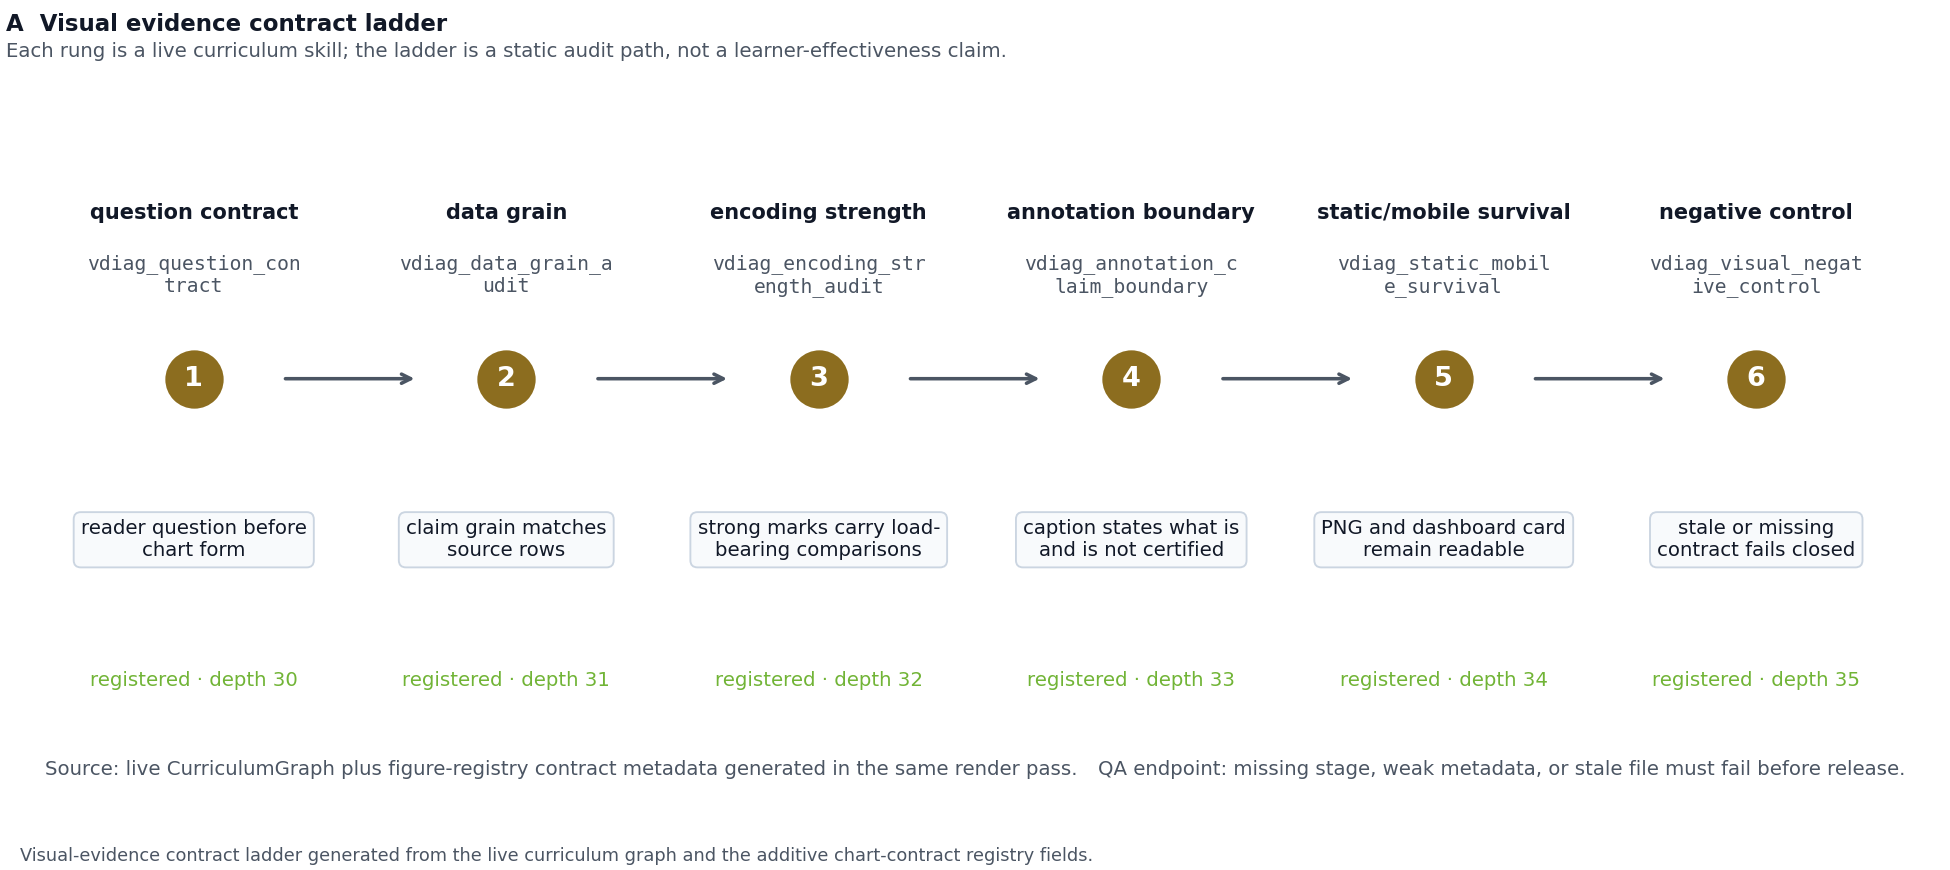
\includegraphics[width=0.98\linewidth,height=0.40\textheight,keepaspectratio,alt={Visual-evidence contract ladder generated from the live curriculum graph and figure registry metadata. Six numbered rungs move from question contract through data grain, encoding strength, annotation boundary, static/mobile survival, and negative-control validation. Each rung names the skill identifier that carries the review obligation and reports whether the skill is registered in the graph. The figure documents the authoring and validation lifecycle for visual evidence; it does not claim learner effectiveness or external deployment performance.}]{../figures/visual_evidence_contract_ladder.png}
\caption{Visual-evidence contract ladder generated from the live
curriculum graph and figure registry metadata. Six numbered rungs move
from question contract through data grain, encoding strength, annotation
boundary, static/mobile survival, and negative-control validation. Each
rung names the skill identifier that carries the review obligation and
reports whether the skill is registered in the graph. The figure
documents the authoring and validation lifecycle for visual evidence; it
does not claim learner effectiveness or external deployment
performance.}\label{fig:visual_evidence_contract_ladder}
\end{figure}

\end{frame}

\begin{frame}[fragile,allowframebreaks]{Citation coverage, locator
health, and evidence-class auditing}
The scientific-claim layer adds one more audit view.
fig.~\ref{fig:scientific_evidence_matrix} is generated from manuscript
\texttt{claim-support} anchors and the support matrix in
\breaktt{data/manuscript\_claim\_support.yaml}. Its rows separate
computed, descriptive-count, simulation, literature, scope-limit,
delivery and visual claims; its columns show whether each class is
backed by claim tokens, manuscript variables, citations, figures,
validators or limitation markers. This is not a statistical result. It
is a release integrity check that prevents strong scientific wording
from passing without a declared evidence class.

\end{frame}

\begin{frame}[fragile,allowframebreaks]{Citation coverage, locator
health, and evidence-class auditing}
\begin{figure}
\centering
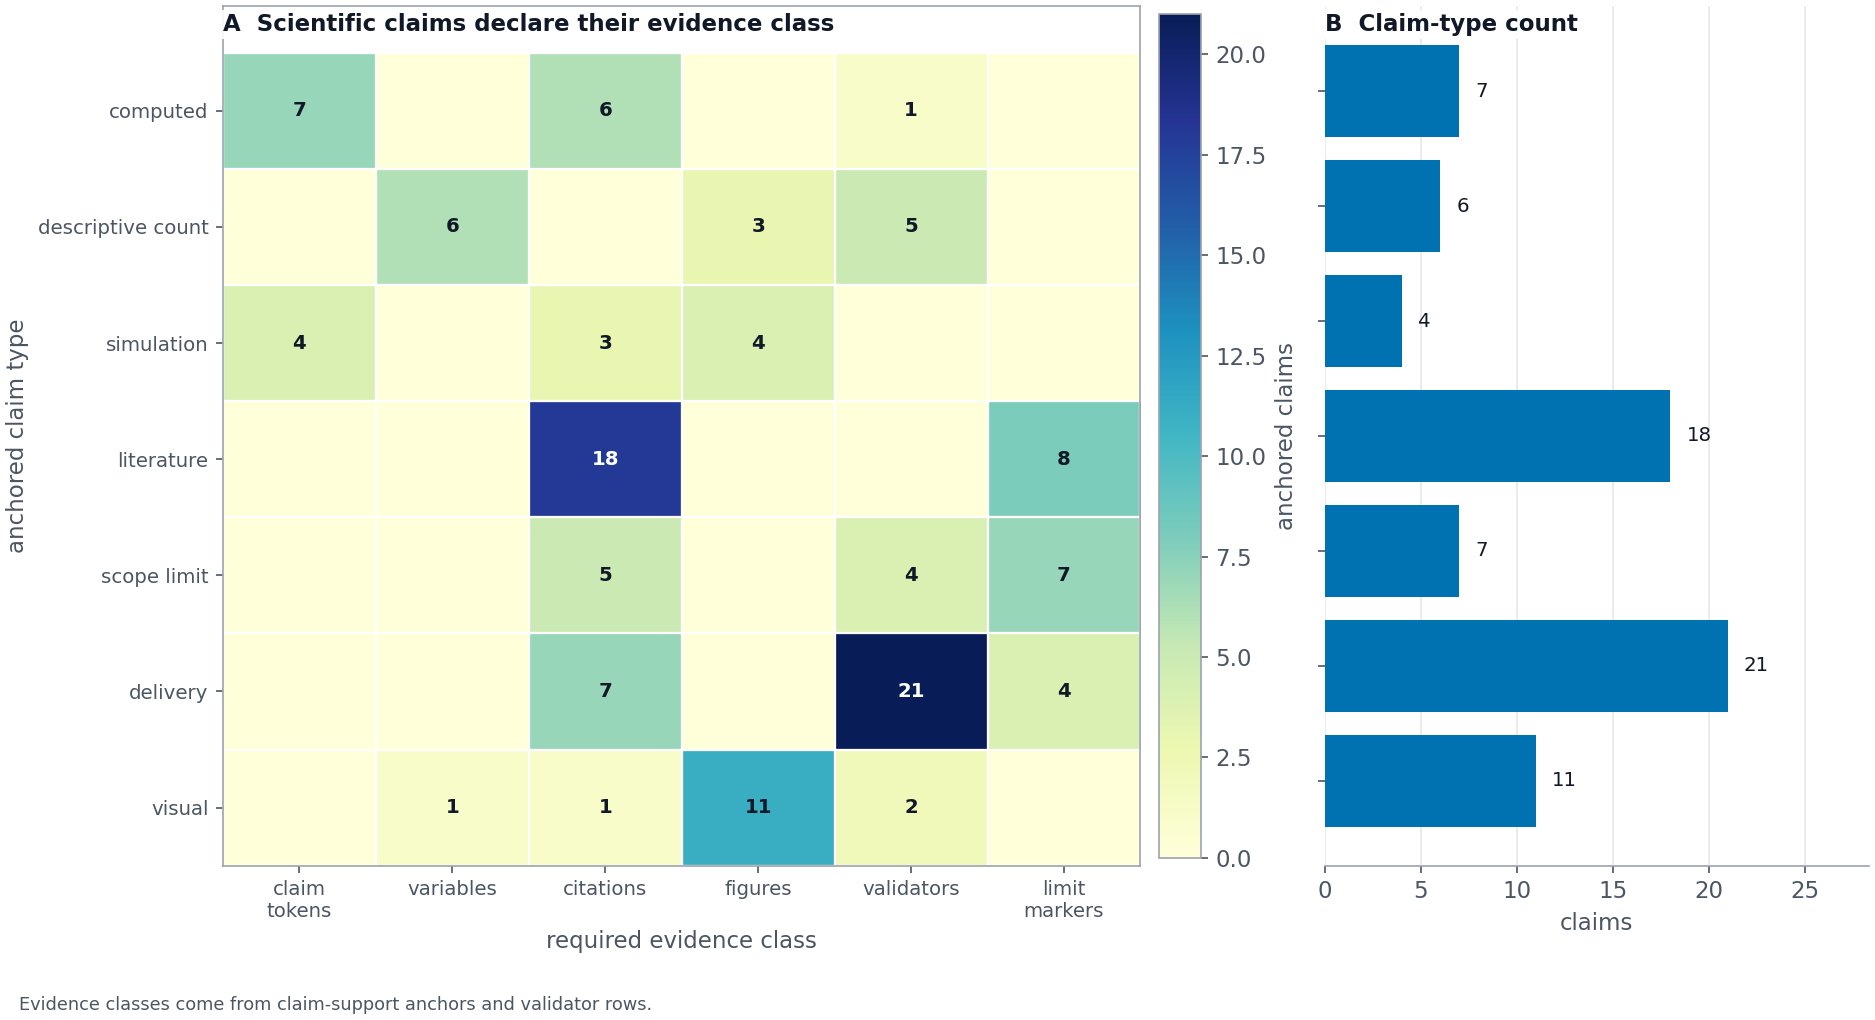
\includegraphics[width=0.96\linewidth,height=0.40\textheight,keepaspectratio,alt={Scientific evidence matrix for manuscript claims generated from claim-support anchors and data/manuscript\_claim\_support.yaml. Rows are claim-support types, columns are evidence classes, cell counts show how many anchored claims use each evidence class, and the side panel counts claims per type. The purpose is epistemic classification rather than statistical inference: computed, descriptive, simulation, literature, scope-limit, delivery, and visual claims are forced to declare the kind of support they actually have.}]{../figures/scientific_evidence_matrix.png}
\caption{Scientific evidence matrix for manuscript claims generated from
claim-support anchors and data/manuscript\_claim\_support.yaml. Rows are
claim-support types, columns are evidence classes, cell counts show how
many anchored claims use each evidence class, and the side panel counts
claims per type. The purpose is epistemic classification rather than
statistical inference: computed, descriptive, simulation, literature,
scope-limit, delivery, and visual claims are forced to declare the kind
of support they actually have.}\label{fig:scientific_evidence_matrix}
\end{figure}

\end{frame}

\begin{frame}[fragile,allowframebreaks]{Citation coverage, locator
health, and evidence-class auditing}
The platform evidence above is intentionally separated from the small
mathematical examples. Those examples are still central teaching
artifacts, but their scientific meaning depends on the supplement's
model assumptions and regime boundaries.
\end{frame}

\end{document}
